\section{Moment Maps of Lie Actions Arising from $\mathrm{SO}(3)$}
Now, we would like to begin developing a generalization of Delzant's  Theorem for a symplectic manifolds admitting a Hamilitonian $\mathrm{SO}(3)$ action, $(M, \omega, \rm{SO}(3))$. 

\begin{remark}
As a result, the moment map for such an action will be $\mu: M \to \mathfrak{so}(3)^{*}$. As a result, we must study the Lie algebra $\mathfrak{so}(3)^{*}$
\end{remark}

\noindent In this section we cover the following: 

\begin{enumerate}
    \item Coadjoint action $\rm{SO}(3)$ is given by evalulation
    \item The Lie-algebra isomorphism $ \mathfrak{so}^{*}(3) \cong \mathbb{R}^{3}$
    \item The classification of moment images of symplectic manifold with Hamilitonian $\mathrm{SO}(3)$ action, $(M, \omega, \rm{SO}(3))$. 
\end{enumerate}

\subsection{Coadjoint Action}

To classify moment map images, we must first show that the natural action of $\rm{SO}(3)$ on $\mathfrak{so}(3)$ is itself given by evaluation. 

\begin{defn}[Coadjoint Action]
Given a Lie group $G$, and its Lie algebra $\mathfrak{g}$, there is a natural action of $G \circlearrowright \mathfrak{g}$ given by the coadjoint action. For each covector $h \in \mathfrak{g}^{*}$, $A \cdot h \to \operatorname{Ad}_{A^{-1}}^{*} h$
\end{defn}

\begin{lemma}\label{lem:so3-isomorphism}
The map $\Phi: \mathfrak{so}(3)^{*} \to \mathbb{R}^{3}$ defined by
\[
\Phi(\xi) = \left( \xi(E_{1}), \xi(E_{2}), \xi(E_{3}) \right)
\]
\noindent is an $\mathrm{SO}(3)$-equivariant vector space isomorphism.
\end{lemma}

\begin{proof}
Since $\dim \mathfrak{so}(3) = \dim \mathfrak{so}(3)^* = 3$, it suffices to show that $\Phi$ is injective. Suppose $\Phi(\xi) = 0$. Then $\xi$ vanishes on the basis $\{E_1, E_2, E_3\}$ of $\mathfrak{so}(3)$, so $\xi = 0$. Hence, $\ker \Phi = 0$, and $\Phi$ is injective.
\end{proof}

\begin{remark}
Now, we would like to prove that the coadjoint action on $\mathfrak{so}(3)^{*}$ is given by evaluation. 
\end{remark}

\begin{lemma}[Coadjoint Action is Given by Evaluation]
\label{ActionEvalulation}
Let $\xi \in \mathfrak{so}(3)^{*}$, and $\Phi$ the evaluation map as above. Then:
\[
\Phi\left( \xi \circ \mathrm{Ad}_{A^{-1}} \right) = A \Phi(\xi)
\]
\end{lemma}

\begin{proof}
Under the isomorphism $\Phi$, and noting that $A^{-1} = A^{T}$ for $A \in \mathrm{SO}(3)$, we want to show \label{AdInvariance} $A \Phi(\xi) = \left( \xi(A^{T} E_{1} A),\; \xi(A^{T} E_{2} A),\; \xi(A^{T} E_{3} A) \right)$. Let $\xi(E_1) = \xi_1$, $\xi(E_2) = \xi_2$, and $\xi(E_3) = \xi_3$. It suffices to verify \eqref{AdInvariance} on the basis elements. We verify this for the first basis element, the other cases follow by a similar computation. 

\begin{align}
\xi \left( A^{T} E_{1} A \right) &= \xi\left(
\begin{bmatrix}
a_{11} & a_{12} & a_{13} \\
a_{21} & a_{22} & a_{23} \\
a_{31} & a_{32} & a_{33}
\end{bmatrix}^{\!\!\!T}
E_{1}
\begin{bmatrix}
a_{11} & a_{12} & a_{13} \\
a_{21} & a_{22} & a_{23} \\
a_{31} & a_{32} & a_{33}
\end{bmatrix}
\right) \\[1em]
&= \xi\left(
\begin{bmatrix}
0 & -a_{21} a_{32} + a_{31} a_{22} & -a_{21} a_{33} + a_{31} a_{23} \\
-a_{22} a_{31} + a_{21} a_{32} & 0 & -a_{22} a_{33} + a_{32} a_{23} \\
-a_{23} a_{31} + a_{21} a_{33} & -a_{23} a_{32} + a_{22} a_{33} & 0
\end{bmatrix}
\right)
\end{align}

\noindent We compute this as a linear combination of the basis matrices:
\begin{align}
\xi(A^{T} E_{1} A) &= 
\det\begin{bmatrix}
a_{22} & a_{23} \\
a_{32} & a_{33}
\end{bmatrix} \xi(E_{1}) +
\det\begin{bmatrix}
a_{22} & a_{32} \\
a_{21} & a_{31}
\end{bmatrix} \xi(E_{2}) +
\det\begin{bmatrix}
a_{21} & a_{22} \\
a_{31} & a_{32}
\end{bmatrix} \xi(E_{3}) \\[0.5em]
&= \det
\begin{bmatrix}
\xi_1(E_{1}) & \xi_2(E_{2} & \xi_3(E_{3}) \\
a_{21} & a_{22} & a_{23} \\
a_{31} & a_{32} & a_{33}
\end{bmatrix} \\[0.5em]
&= \left\langle \Phi(\xi),\; A^{T} e_2 \times A^{T} e_3 \right\rangle 
= \left\langle A \xi,\; e_1 \right\rangle 
= \left[ A \Phi(\xi) \right]_1
\end{align}

\noindent The same holds for components 2 and 3. Therefore,
\[
\Phi \left( \operatorname{Ad}^* A \cdot \xi \right )_j = \left[ A \Phi(\xi) \right] _j
\quad \text{for } j = 1, 2, 3
\]

\noindent 
\end{proof}

\noindent \textbf{References: } \textcite{Blaom1996}

\subsection{Lie Algebra of $\mathfrak{so}(3)$}

Now, we have found the the coadjoint action $\operatorname{Ad}_{A^{-1}}^{*}$, is given by evalulation. Now, we would like to develop the Lie algebra isomorphism between $(\mathbb{R}^{3}, \times)$ and $(\mathfrak{so}(3), [\cdot, \cdot])$. This isomorphism will allow us to interpert the images of moment maps $\mu: M \to \mathfrak{so}(3)^{*}$ as though they were in Euclidean space. 

\begin{remark}[Lie algebra of $\mathfrak{so}^{3}$]
The Lie algebra of $\mathfrak{so}^{3}$ has the Lie bracket given by the matrix commutator. Therefore, we denote the Lie algebra as $(\mathfrak{so}_{3}$.  Furthermore,  The Lie algebra of $\mathbb{R}^{3}$ has the Lie bracket given by the cross product. Therefore, we denote the Lie algebra as $(\mathbb{R}^{3}, \times)$. 
\end{remark}

\begin{lemma}[Lie Algebra Isomorphism]
\label{LieAlgebraIso}
$(\mathbb{R}^{3}, \times) \to (\mathfrak{so}(3), [\cdot, \cdot])$ given by 

\begin{align}
\phi: (x_1, x_{2}, x_{3}) \to 
\begin{bmatrix}
0 & -x_3 & x_2 \\
x_3 & 0 & -x_1 \\
-x_2 & x_1 & 0
\end{bmatrix}
\in \mathfrak{so}(3) 
\end{align}

\noindent is an isomorphism of Lie algebras
\end{lemma}

\begin{proof}
Note that $\phi$ is injective. Furthermore, we note that $\dim \mathfrak{so}(3) = \mathbb{R}^3$. Therefore, we know that $\phi$ is an isomorphism of vector spaces. Now, we show that Lie bracket is preserved under isomorphism. Let $X = (x_{1}, x_{2}, x_{3})$, and $Y = (y_{1}, y_{2}, y_{3})$. Then, we note that:

$$[X,Y] = X \times Y = (x_{2} y_{3} - x_{3} y_{2}, x_{3} y_{1} - y_{3} x_{1}, x_{1} y_{2} - y_{1} x_{2})$$

\noindent Therefore, we have that 

$$\phi([X,Y]) = \begin{bmatrix}
0 & -x_{1} y_{2} + y_{1} x_{2} & x_{3} y_{1} - y_{3} x_{1} \\
x_{1} y_{2} - y_{1} x_{2} & 0 & -x_{2} y_{3} + x_{3} y_{2} \\
-x_{3} y_{1} + y_{3} x_{1} & x_{2} y_{3} - x_{3} y_{2} & 0
\end{bmatrix}$$

\noindent Alternatively, when we compute 

$$[\phi(X), \phi(Y)] = \phi(X) \phi(Y) - \phi(Y) \phi(X)$$

\noindent We notice that the following occurs: 

$$[\phi(X), \phi(Y)]  = \begin{bmatrix}
0 & -x_3 & x_2 \\
x_3 & 0 & -x_1 \\
-x_2 & x_1 & 0
\end{bmatrix} \begin{bmatrix}
0 & -y_3 & y_2 \\
y_3 & 0 & -y_1 \\
-y_2 & y_1 & 0
\end{bmatrix} - \begin{bmatrix}
0 & -y_3 & y_2 \\
y_3 & 0 & -y_1 \\
-y_2 & y_1 & 0
\end{bmatrix} \begin{bmatrix}
0 & -x_3 & x_2 \\
x_3 & 0 & -x_1 \\
-x_2 & x_1 & 0
\end{bmatrix} $$

$$= \begin{bmatrix}
0 & -x_{1} y_{2} + y_{1} x_{2} & x_{3} y_{1} - y_{3} x_{1} \\
x_{1} y_{2} - y_{1} x_{2} & 0 & -x_{2} y_{3} + x_{3} y_{2} \\
-x_{3} y_{1} + y_{3} x_{1} & x_{2} y_{3} - x_{3} y_{2} & 0
\end{bmatrix}$$

\noindent Therefore, we conclude.
\end{proof}

\begin{remark}
As a consequence, this will establish that there is a Lie algebra isomorphism between $(\mathfrak{so}(3)^{*}, [\cdot, \cdot])$ and $(\mathbb{R}^{3}, \times)$ as well. 
\end{remark}

\begin{remark}
Now, there exists a Lie algebra isomorphism between $\mathfrak{so}(3)^{*}$ and $\mathbb{R}^{3}$ by chasing the diagram: 
\end{remark}

\[
\begin{tikzcd}
\mathbb{R}^3 \arrow[r, "\phi"] & \mathfrak{so}(3) \arrow[d] \\
\mathbb{R}^3 \arrow[u] & \mathfrak{so}(3)^* \arrow[l, "\Phi"]
\end{tikzcd}
\]

\begin{remark}
Now, we study the images of $\mu$ moment maps arising from a Hamilitonian $\rm{SO}(3)$-action on $(M, \omega, \rm{SO}(3))$. We use the above results freely \ref{ActionEvalulation}, and \ref{LieAlgebraIso}
\end{remark}

\subsection{Images of Moment Maps}

Now, we define a specific notion of equivariance

\begin{defn}[$G$-Equivariance]
Let $G$ be a Lie group action both on $G \circlearrowright X$ and on $G \circlearrowright Y$. Let $f: X \to Y$ a diffeomorphism. Then $f$ is $G$-equivariant if:

$$f(g \cdot x) = \phi(g) \cdot f(x)$$
\end{defn}

\noindent Consider a symplectic manifold $(M, \omega, \rm{SO}(3))$, with moment map $\mu: M \to \mathfrak{so}_{3}^{*}$. We  show a useful lemma, that is coadjoint action acts equivariantly on the moment map. This will allow us to control the moment map image. 

\begin{lemma}[Coadjoint Action is $A$-Equivariant]
Consider a connected symplectic manifold $(M, \omega, \rm{SO}(3))$, and $A \in \rm{SO}(3)$. Then, we have that:

$$\mu(A \cdot x) =  Ad_{A^{-1}}^{*} \mu(x)$$

\noindent where $Ad_{A^{-1}}^{*}$ denotes the pullback. 
\end{lemma}

\begin{proof}
It is enough to prove the differential identity on both sides. Namely, observe that the above statement is equivalent to:
$$d \mu_{x} (X^{\#}_{M}|_{x}) =  \mu(x) \circ \operatorname{ad}(-X, \cdot)$$
Now, consider $Y \in \mathfrak{so}(3)$. Then, we note that 
\begin{align}
\mu_{x} (X^{\#}_{M}|_{x}) Y = \omega_{x}(X^{\#}_{M}|_{x}, Y^{\#}_{M}|_{x}) = \{\mu^X, \mu^Y \} = \mu^{[X,Y]}(x) = \mu(x)[Y, X]
\end{align}
Now, we manipulate the expression $\mu(x) \circ \operatorname{ad}(-X, \cdot)$, and find: 
\begin{align}
\left[ \mu(x) \circ ad(-X, \circ) \right] Y = \mu(x)[-X,Y] = \mu(x)[Y,X]
\end{align}
Since both expressions agree on the differential level, the conclusion follows. 
\end{proof}

Now, since the coadjoint action is $A$-Equivariant, and the coadjoint action is given by evaluations, we have that $\mu$ is $\rm{SO}(3)$ invariant. Now, we use that $\mathfrak{so}(3)^{*} \cong \mathbb{R}^{3}$ to invoke that images of moment maps $\mu: M \to \mathbb{R}^{3}$ must have $\mathrm{SO}(3)$ symmetry. \bigskip  

\noindent \textbf{References}: \textcite{Terek2020}

\subsection{Sets that are $\mathrm{SO}(n)$ Invariant}

\begin{lemma}\label{lem:so-invariant-subsets}
Let $\mathrm{SO}(n)$ act on $\mathbb{R}^{n}$ by the standard action, and let $K \subset \mathbb{R}^{n}$ be $\mathrm{SO}(n)$-invariant. We define $\|K\| = \{\|w\|: w \in K \}$.
Then:
\begin{equation}
K = \bigcup_{r \in \|K\|} S^{n-1}(r)
\end{equation}
If $K$ is connected, in particular, one of the following occurs  
\begin{enumerate}
    \item $K = \emptyset$
    \item $K = S^{n-1}(r)$ for some $r > 0$
    \item $K = \{x \in \mathbb{R}^{n}: \|x\| \leq r\}$ for some $r > 0$
    \item $K = \{x \in \mathbb{R}^{n}: r_{1} \leq \|x\| \leq r_{2}\}$ for $0 < r_1 < r_2$
\end{enumerate}
\end{lemma}
\begin{proof}
We observe that for each $p \in \mathbb{R}^{n}$:
\begin{equation}
\mathrm{SO}(n) \cdot p = \{y \in \mathbb{R}^n : \|y\| = \|p\|\}
\end{equation}
Therefore, as $p \in K$, it holds that $\mathrm{SO}(n) \cdot p \subset K$. So:
\begin{equation}
\bigcup_{r \in \|K\|} S^{n-1}(r) = \bigcup_{p \in K} \mathrm{SO}(n) \cdot p \subset K
\end{equation}
The reverse inclusion follows from the observation that if $w \in K$, then $\|w\| \in \|K\|$ and $w \in S^{n-1}(\|w\|)$. Now, by continuity of the norm function $x \mapsto \|x\|$, if $K$ is compact and connected, so will be $\|K\|$. Therefore, $\|K\| = [r_{1}, r_{2}]$ where $0 \leq r_{1} \leq r_{2} < \infty$.
\end{proof}
\begin{theorem}\label{thm:minkowski-sum-spheres}
Let $r_{1}, r_{2} \in [0, \infty)$ such that $r_{1} < r_{2}$. Then:
\begin{equation}
S^{n-1}(r_{1}) + S^{n-1}(r_{2}) = \bigcup_{r \in [r_{2} - r_{1}, r_{2} + r_{1}]} S^{n-1}(r)
\end{equation}
where the sum on the left is the Minkowski sum of the two spheres 
\end{theorem}
\begin{proof}
If $y \in S^{k}(r_{1}) + S^{k}(r_{2})$ then $y = x_{1} + x_{2}$ where $x_{1} \in S^{k}(r_{1})$ and $x_{2} \in S^{k}(r_{2})$. By the triangle inequality:
\begin{equation}
r_{2} - r_{1} = \|x_{2}\| - \|x_{1}\| \leq \|y\| \leq \|x_{2}\| + \|x_{1}\| = r_{2} + r_{1}
\end{equation}
Therefore,
\begin{equation}
y \in \bigcup_{r \in [r_{2} - r_{1}, r_{2} + r_{1}]} S^{k}(r)
\end{equation}
For the other inclusion, by $\mathrm{SO}(k+1)$ invariance, we conclude without loss of generality that $k=1$. By $\mathrm{SO}(2)$ invariance, we further assume that $y = (0,r)$ with $r \in [r_{2} - r_{1}, r_{2} + r_{1}]$. If:
\begin{align}
x_{1} &= (r_{1} \sin \theta_{1}, r_{1} \cos \theta_{1})\\
x_{2} &= (r_{2} \sin \theta_{2}, r_{2} \cos \theta_{2})
\end{align}
The condition $r \in [r_{2} - r_{1}, r_{2} + r_{1}]$ means that there are $\theta_{1}$ and $\theta_{2}$ such that:
\begin{align}
r_{2} \sin \theta_{2} + r_{1} \sin \theta_{1} &= 0\\
r_{2} \cos \theta_{2} + r_{1} \cos \theta_{1} &= r
\end{align} \end{proof}
\begin{figure}[htbp]
    \centering
    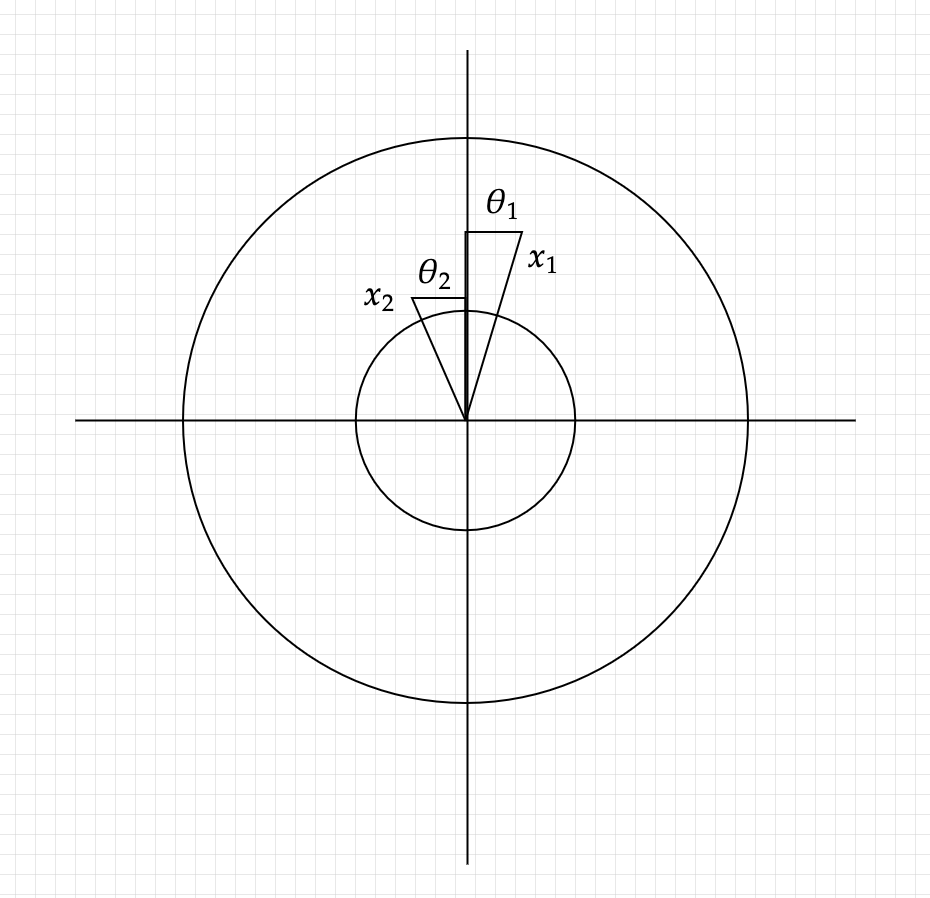
\includegraphics[width=0.3\linewidth]{Chapters/Figures/Screenshot 2025-04-01 at 10.48.42 AM.png}
    \caption{Geometric visualization of the Minkowski sum of two spheres $S^{n-1}(r_1)$ and $S^{n-1}(r_2)$, showing how the resulting set forms a spherical shell with inner radius $r_2-r_1$ and outer radius $r_2+r_1$.}
    \label{fig:sphere-minkowski-sum}
\end{figure}

\noindent This geometric interpretation of the Minkowski sum of spheres is fundamental for understanding the structure of moment-image sets for Hamiltonian $\mathrm{SO}(3)$-spaces. Now, we can classify all possible moment-images of compact connected Hamiltonian $\mathrm{SO}(3)$-spaces as being one of four types: a point (the origin), a sphere, a solid ball, or a spherical shell. \bigskip 

\noindent \textbf{References}: \textcite{Terek2020}

\newpage 
\setcounter{section}{6}